%%%%%%%%%%%%%%%%%%%%%%%%%%%%%%%%%%%%

\section{2標本検定の検出力の計算}

%%%%%%%%%%%%%%%%%%%%%%%%%%%%%%%%%%%%

\begin{frame}
\frametitle{}

\begin{center}
\begin{tabular}{l l | c c}
\multicolumn{2}{c}{} & \multicolumn{2}{c}{\textbf{決定}} \\
& & $H_0$を棄却しない &  $H_0$を棄却する \\
  \cline{2-4}
& $H_0$が真 & \green{$1 - \alpha$} & \orange{第一種の過誤，$\alpha$} \\
\raisebox{1.5ex}{\textbf{真実}} & $H_A$が真 &  \orange{第二種の過誤，$\beta$} & \green{検出力，$1 - \beta$} \\
  \cline{2-4}
\end{tabular}
\end{center}

\begin{itemize}
\item 第一種の過誤は$H_0$を誤って棄却することであり、その確率は$\alpha$（有意水準）である。

\item 第二種の過誤は$H_0$を棄却すべきときに棄却しないことであり、その確率は$\beta$（計算は少し複雑）である。

\item 検定の\hl{検出力}は$H_0$を正しく棄却する確率であり、その確率は$1 - \beta$である。

\item 仮説検定では$\alpha$と$\beta$を低く保ちたいが、両者の間にはトレードオフが存在する。

\end{itemize}

\end{frame}

%%%%%%%%%%%%%%%%%%%%%%%%%%%%%%%%%%%%

\begin{frame}
\frametitle{第二種の過誤の確率}

対立仮説が実際に真である場合、第二種の過誤（棄却すべきときに帰無仮説を棄却しない）を犯す可能性はどれくらいか？

\begin{itemize}

\item 答えは自明ではない。

\item 真の母集団平均が帰無仮説の値に非常に近い場合、差を検出する（$H_0$を棄却する）のが難しい。

\item 真の母集団平均が帰無仮説の値から大きく離れている場合、差を検出しやすい。

\item 明らかに、$\beta$は\hl{効果量}（$\delta$）に依存する。
\end{itemize}

\end{frame}

%%%%%%%%%%%%%%%%%%%%%%%%%%%%%%%%%%%%

\begin{frame}
\frametitle{例 - 血圧（BP）：仮説}

{\dq
{\footnotesize
ある製薬会社が血圧を下げる新薬を開発し、臨床試験でその有効性を検証しようとしているとする。特定の標準的な血圧薬を服用している人々を募集し、被験者の半分に新薬（治療群）を投与し、残りの半分には外見が同じプラセボで現在の薬を継続服用させる（対照群）。この文脈での両側仮説検定の仮説は何か？
}
}

\soln{
\begin{align*}
H_0&: \mu_{\text{治療群}} - \mu_{\text{対照群}} = 0 \\
H_A&: \mu_{\text{治療群}} - \mu_{\text{対照群}} \ne 0
\end{align*}
}

\end{frame}

%%%%%%%%%%%%%%%%%%%%%%%%%%%%%%%%%%%%

\begin{frame}
\frametitle{例 - BP：標準誤差}

{\dq
{\footnotesize
研究者は収縮期血圧が140から180 mmHgの患者を対象に臨床試験を行うとする。以前発表された研究によれば、患者の血圧の標準偏差は約12 mmHgで、分布はほぼ対称であるとする。グループごとに100人の患者がいる場合、治療群と対照群の標本平均の差の近似標準誤差はどれくらいか？
}
}

\soln{
\[ SE = \sqrt{ \frac{12^2}{100} + \frac{12^2}{100} } = 1.70 \]
}

\end{frame}

%%%%%%%%%%%%%%%%%%%%%%%%%%%%%%%%%%%%

\begin{frame}
\frametitle{例 - BP：$H_0$を棄却するために必要な最小効果量}

{\dq
{\footnotesize
5\%の有意水準で帰無仮説を棄却するためには、治療群と対照群の観察された血圧平均の差（効果量）はどの値である必要があるか？}
}

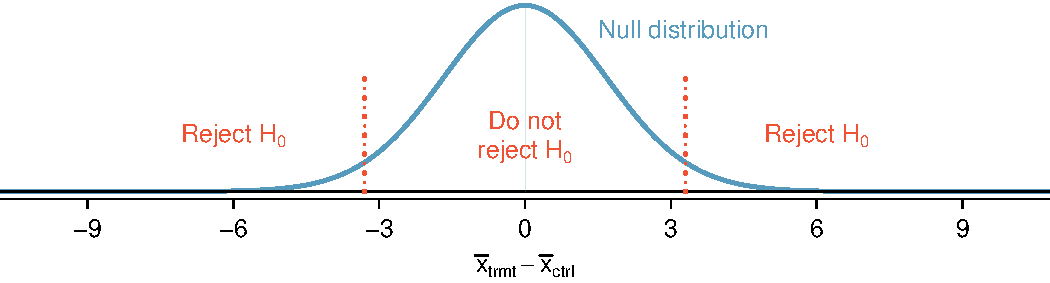
\includegraphics[width=\textwidth]{7-4_power/figures/power/power_null_B_0_1-7_with_rejection_region}

差は少なくとも
\[ 1.96 \times 1.70 = 3.332 \]
または多くとも
\[ -1.96 \times 1.70 = -3.332 \]
である必要がある。

\end{frame}

%%%%%%%%%%%%%%%%%%%%%%%%%%%%%%%%%%%%

\begin{frame}
\frametitle{例 - BP：検出力}

{\dq
{\footnotesize
研究者が標準薬と比べて3 mmHg以上の血圧への影響を検出することに関心があるとする。この効果を検出できる検定の検出力はどれくらいか？
}}

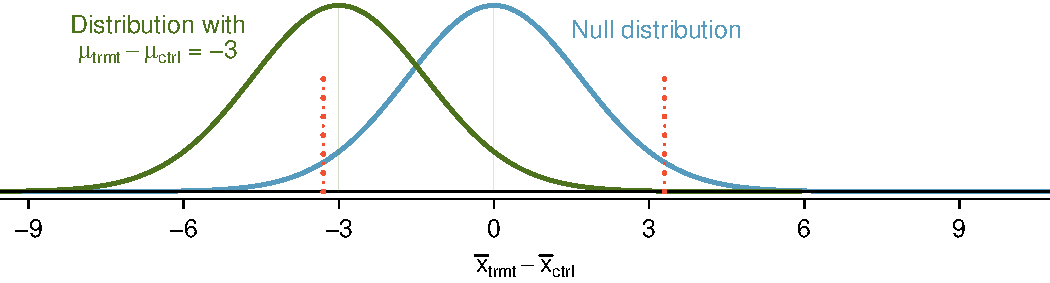
\includegraphics[width=\textwidth]{7-4_power/figures/power/power_null_C_0_1-7_with_alt_at_3}

\[ Z = \frac{-3.332 - (-3)}{1.70} = -0.20 \]

\[ P(Z < -0.20) = 0.4207 \]

\end{frame}

%%%%%%%%%%%%%%%%%%%%%%%%%%%%%%%%%%%%

\begin{frame}
\frametitle{例 - BP：80\%の検出力に必要な標本サイズ}

{\dq
{\footnotesize
この検定で80\%の検出力を得るためにはどれくらいの標本サイズが必要か？
}}

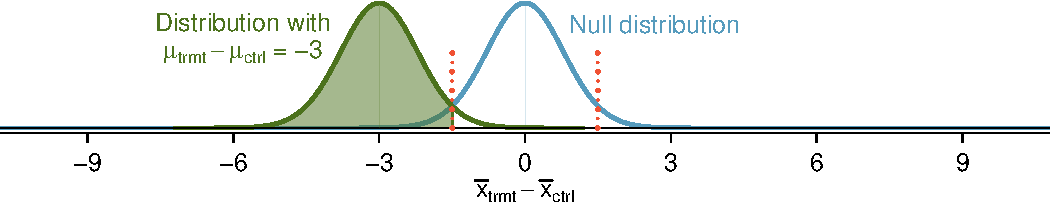
\includegraphics[width=\textwidth]{7-4_power/figures/power/power_null_0_0-76_with_alt_at_3_and_shaded}

\[ SE = \frac{3}{2.8} = 1.07142 \]

\[ 1.07142 = \sqrt{ \frac{12^2}{n} + \frac{12^2}{n} } \]

\[ n = 250.88 \rightarrow n \ge 251 \]

\end{frame}

%%%%%%%%%%%%%%%%%%%%%%%%%%%%%%%%%%%%

\begin{frame}
\frametitle{まとめ}

\begin{itemize}
\item 目標の検出力のレベルに必要な標本サイズを計算する。
\item 様々な標本サイズに対して検出力を計算し、目標の検出力（通常80\%または90\%）が得られる標本サイズを選ぶ。
\end{itemize}
\begin{center}
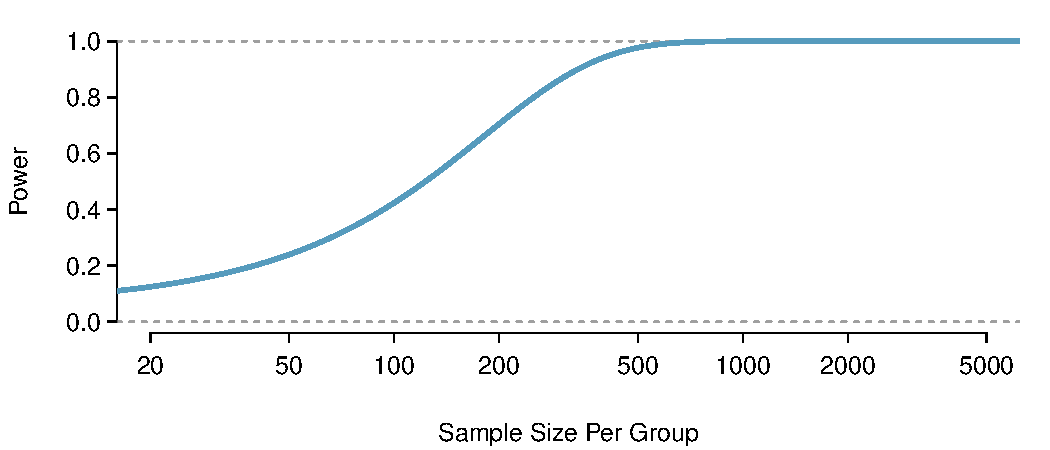
\includegraphics[width=0.7\textwidth]{7-4_power/figures/power/power_curve_neg-3}
\end{center}

\end{frame}

%%%%%%%%%%%%%%%%%%%%%%%%%%%%%%%%%%%%

\begin{frame}
\frametitle{望ましい検出力を達成する方法}

検出力を高める（第二種の過誤率を下げる）方法はいくつかある：

{\small
\begin{enumerate}

\item 標本サイズを増やす。

\item 標本の標準偏差を減らす。これは実質的に標本サイズを増やすのと同じ効果をもたらす（標準誤差が小さくなる）。$s$が小さいほど、帰無値と観察された点推定量を区別しやすくなる。確保するのは難しいが、慎重な測定プロセスと母集団をより均質に限定することで助けになる場合がある。

\item $\alpha$を増やすことで$H_0$を棄却しやすくする（ただし、これには第一種の過誤率が増加するという副作用がある）。

\item より大きな効果量を考慮する。母集団の真の平均が対立仮説にあるが帰無値に近い場合、差を検出するのが難しくなる。

\end{enumerate}
}

\end{frame}

%%%%%%%%%%%%%%%%%%%%%%%%%%%%%%%%%%%%
